\documentclass{article}
\usepackage[T1]{fontenc}
\usepackage[polish]{babel}
\usepackage[utf8]{inputenc}
\usepackage{listings}
\usepackage{graphicx}
\usepackage[margin=1in]{geometry}
\title{Kryptografia 2023 Exercise 5 List 1}
\author{Jakub Patałuch}

\begin{document}

\section{Zadanie 1}
\subsection{Model}
\subsubsection{Parametry}
\begin{itemize}
    \item $N$ - rozmiar macierzy
    \item $A_{ij} = \frac{1}{i+j-1}$ dla $i,j={1,\cdots,N} $ - macierz
    \item $b_i = \sum_{j=1}^{N} \frac{1}{i+j-1}$ dla $i = {1,\cdots,N}$ - wektor prawych stron
    \item $c_i = \sum_{j=1}^{N} \frac{1}{i+j-1}$ dla $i = {1,\cdots,N}$ - wektor kosztów
\end{itemize}

\subsubsection{Zmienne decyzyjne}
\begin{itemize}
    \item $X_1, \cdots X_{N}$ - rozwiazania równania $AX=b$
\end{itemize}

\subsubsection{Ograniczenia}
\begin{enumerate}
    \item $\forall_{i=1}^{n} (\sum_{j=1}^{N} A_{ij} * X_{j} = b_{i})$ - równanie jest spełnione
\end{enumerate}

\subsubsection{Funkcja celu}
\[min \sum_{i=1}^{N} X_{i} * c_{i}\]

\subsection{Wyniki}
Błąd względny dla zadanego $N$ prezentuje się następująco:

\begin{center}
    \begin{tabular}{| c | c |}
        \hline
        N & Błąd względny \\ \hline
        1 & 0 \\ \hline
        2 & 0 \\ \hline
        3 & 0 \\ \hline
        4 & 0 \\ \hline
        5 & 0 \\ \hline
        6 & 0 \\ \hline
        7 & 0 \\ \hline 
        8 & 0.514059 \\ \hline
        9 & 0.682911 \\ \hline 
        10 & 0.990388 \\ \hline
    \end{tabular}
\end{center}

Macierz hilberta jest źle uwarunkowana.

\section{Zadanie 2}
\subsection{Model}
\subsubsection{Parametry}
\begin{itemize}
    \item $Types := \{"Typ 1", "Typ 2"\}$ - zbiór rodzajów dzwigów 
    \item $Sites$ - zbiór lokacji 
    \item $(\forall_{s \in Sites} \forall_{t \in Types}) Excess_{s,t} \ge 0$ - Nadmiar dźwigu typu $t$ w lokacji $s$.
    \item $(\forall_{s \in Sites} \forall_{t \in Types}) Deficit_{s,t} \ge 0$ - Niedomiar dźwigu typu $t$ w lokacji $s$.
    \item $(\forall_{s \in Sites} \forall_{d \in Sites}) Distance_{s,d} \ge 0$ - Odległość od lokacji $s$ do lokacji $d$.
    \item $(\forall_{t \in Types}) TransportationCost_{t} \ge 0$ - Koszt transportu dla dźwigu typu $t$ zależnie od odległości.
\end{itemize}
Ze względu na możliwość zastąpienia dźwigu typu 1, dźwigiem typu 2, rodzaje dźwigów nie mogę być sparametryzowane.
\subsubsection{Zmienne decyzyjne}
\begin{itemize}
    \item $(\forall_{t \in Types} \forall_{src \in Sites} \forall_{dst \in Sites})MoveTo_{t,src,dst}$ - ilość dźwigów typu $t$ 
        przeniesiona z lokacjizacji $src$ do $dst$.
\end{itemize}

\subsubsection{Ograniczenia}
\begin{enumerate}
    \item $(\forall_{src \in Sites} \forall_{t \in Types}) \sum_{dst \in Sites} MoveTo_{t,src,dst} <= Excess_{src,t}$ -
        z lokacji $src$ nie wywieziono więciej dźwigów typu $t$ niż ich nadmiar.
    \item $(\forall_{dst \in Sites})\sum_{src \in Sites} MoveTo_{"Typ 2", src, dst} >= Deficit_{dst,Typ2}$ - do każdej
    lokacji przywieziono nie mniej niż deficyt dźwigów typu 2. 
    \item $(\forall_{dst \in Sites}) \sum_{t \in Types, src \in Sites} MoveTo_{t,src,dst} == \sum_{t \in Types} Deficit_{dst, t}$
        - suma przywiezionych dźwigów obu typów jest równa sumie brakujących dźwigów obu typu.
\end{enumerate}

Czy z ograniczeń wynika że zostanie spełnione zaptrzebowania na dźwigu obu typów i można zastąpić dźwig typu 1, dźwigiem typu 2?

Niech dla $dst \in Sites$, $In_1, In_2$ odpowiadają sumie dostarczonych dźwigów typu 1 i 2 do tej lokacji oraz $N_1, N_2$ odpowiadają
potrzebie dźwigów w tej lokalizacji. Z ograniczenia 2 wiemy że:
\[In_2 \ge N_2\]
czyli $\exists e \ge 0$ takie że
\[In_2 = N_2 + e_2\]
Z ograniczenia 3:
\[In_1 + In_2 = N_1 + N_2\]
\[In_1 + N_2 + e_2 = N_1 + N_2\]
\[In_1 + e_2 = N_1\]
Ilość dostarczonych dźwigów 1 typu plus pewna ilość nadmiarowych dźwigów 2 typu równa się wymaganej liczbie dźwigów 1 typu.

\subsubsection{Funkcja celu}

\[min \sum_{t \in Types} \sum_{src \in Sites, dst \in Sites} MoveTo_{t,src,dst} * Distance_{src,dst} * TransportationCost_{t}\]

\subsection{Wyniki}

\begin{center}
    \begin{tabular}{| c | c | c | c | c | c | c | c |}
        \hline
                & Opole & Brzeg & Nysa &  Prudnik & Strzelce Opolskie &  Kozle &  Raciborz\\ \hline
        Opole   & (0,0) & (0,0) & (0,2) & (0,0) & (0,0) & (0,0) & (0,0) \\ \hline
        Brzeg   & (0,0) & (0,1) & (5,0) & (0,0) & (4,0) & (0,0) & (0,0) \\ \hline
        Nysa    & (0,0) & (0,0) & (0,0) & (0,0) & (0,0) & (0,0) & (0,0) \\ \hline
        Prudnik & (0,0) & (0,0) & (0,0) & (0,3) & (1,0) & (0,0) & (0,0) \\ \hline
        Strzelce Opolskie       & (0,0) & (0,0) & (0,0) & (0,4) & (0,0) & (0,0) & (0,0) \\ \hline
        Kozle   & (7,0) & (0,0) & (1,0) & (0,2) & (0,0) & (0,0) & (0,0) \\ \hline
        Raciborz        & (0,0) & (0,0) & (0,0) & (0,1) & (0,0) & (0,0) & (0,0) \\ \hline
    \end{tabular}
\end{center}

Funkcja kosztu = $1818$
Założenie całkowitoliczbowości nie jest potrzebne.

\section{Zadanie 3}
\subsection{Model}
\begin{center}
    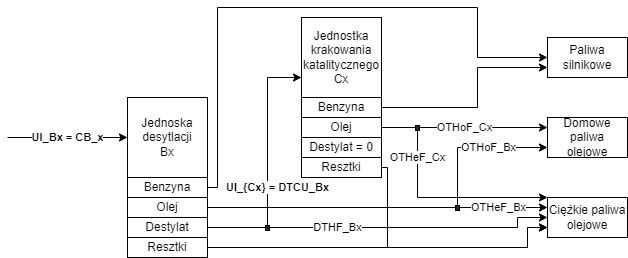
\includegraphics[width = 5in]{model.png}
\end{center}

\subsubsection{Parametry}
\begin{itemize}
    \item $P$ - (Product) zbior dostępnych produktów wyjściowych
    \item $DU$ - (Distillation Unit) zbiór jednosted destylacji
    \item $CU$ - (Cracking Unit) zbiór jednostek krakowania katalitycznego
    \item $AU$ = $DU \cup CU$ - (All Units)
    \item $ (\forall p \in P)(\forall u \in AU) E{p,u} \ge 0$ - wydajność procesu 
        produkcji produktu $p$ na jednostce $u$. 
    \item $ (\forall u \in AU)SC_u$ - (Sulfur Content) zawartość siarki w oleju pochodzącym z danej jednostki $u$
    \item $SCL$ - (Sulfur Content Limit) maksymalna zawartość siarki w oleju przeznaczonym do użytku
        w domowych paliwach olejowych.
    \item $EFD$ - (Engine Fuel Demand) wymagana ilość paliw silnikowych
    \item $HoFD$ - (Home Fuel Demand) wymagana ilość domowych paliw olejowych
    \item $HeFD$ - (Heavy Feal Demand) wymagana ilość ciężkich paliw olejowych
    \item $ (\forall u \in AU) PC_u $ - (Production Cost) koszt przetworzenia jednej tony materiałów w jednostce $u$
    \item $ (\forall d \in DU) COC_d $ - (Crude Oil Cost) kosz kupienia tony ropy do jednostki destylacji $d$.
\end{itemize}

\subsubsection{Zmienne decyzyjne}
\begin{enumerate}
    \item $(\forall u \in AU) UI_u \ge 0$ - (UnitInput), ilość surowych materiałów wchodzących do jednostki $u$
    \item $(\forall u \in AU) OTHoF_u \ge 0$ - (Oil To Home Fuels), ilość oleju produkowanego w jednostce $u$, który
        jest przyporządkowana olejowym paliwom domowym.
    \item $(\forall u \in AU) OTHeF_u \ge 0$ - (Oil to Heavy Fuels), ilość oleju produkowanego w jednostce $u$, który
        jest przyporządkowana ciężkim paliwom olejowym.
    \item $(\forall d \in DU) DTCU_d \ge 0$ - (Distillat to Cracking Unit), ilość destylatu produkowanego w jednostce $d$,
        który wysyłany jest do dalszego przetwarzania w jednostce krakowania katalitycznego
    \item $(\forall d \in DU) DTHF_d \ge 0$ - (Distillat to Heavy Fuel), ilość destylatu produkowanego w jednostce $d$,
        który przyporządkowany ciężkim paliwom olejowym
\end{enumerate}

\subsubsection{Ograniczenia}
\begin{enumerate}
    \item $(\forall u \in AU) OTHoF_u + OTHeF_u == UI_u * E_{Oil, u}$ - dla każdej jednostki produkcyjnej, suma oleju
        przyporządkowanego do paliw domowych i do paliw ciężkich jest równa ilości wyprodukowanego oleju
    \item $(\forall d \in DU) DTCU_d + DTHF_d == UI_d * E_{Distillat, d}$ - dla każdej jednostki destylacji, ilość destylatu
        przekazanego do paliw ciężkich i do jednostek krakowania katalitycznego jest równa ilość wyprodukowanego destylatu
    \item $ \sum_{u \in AU}( UI_u * E_{Benzyna, u}) \ge EFD$ - wyprodukowano wymaganą ilość paliw silnikowych 
    \item $ \sum_{u \in AU}(OTHoF_u) \ge HoFD$ - wyprodukowano wymaganą ilość domowych paliw olejowych
    \item $ \sum_{u \in AU}( Ui_u * E_{Resztki,u} + OTHeF_u) + \sum_{d \in DU} DTHF_d \ge HeFD$ - wyprodukowano wymaganą ilość ciężkich 
        paliw olejowych
    \item $ \sum_{u in AU} OTHoF_u * (SC_u - SCL) \le 0 $ - zawartość siarki w domowych paliwach olejowych nie przekracza limitu
\end{enumerate}

Jako, że powyższy model jest uogólniony, musimy zawęzić go dodatkowymi ograniczeniami:

\begin{enumerate}
    \item $ (\forall c \in CU) OTHeF_c = 0 $ - olej z jendostki krakowania katalitycznego może być użyty tylko
        jako domowe paliwo olejowe.
    \item $ UI_{C1} = DTCU_{B1} \land UI_{C2} = DTCU_{B2} $ - ilość surowych materiałów na wejście jednostek krakujących
        odpowiada ilości destylatu przekazanej do jednostki krakującej z odpowiadającej jednostki destylacji
\end{enumerate}

\subsubsection{Funkcja celu}
\[min \sum_{u \in AU}(UI_u * PC_u) + \sum_{d \in DU}(UI_d * COC_d)\]

\subsection{Wyniki}
Dla naszych danych:
\begin{center}
    \begin{tabular}{| c | c | c |} \hline
    Var & $B1$ & $B2$ \\ \hline
    $UI$ & 1075601.374570 & 0 \\ \hline
    $DTCU$ & 77319.587629 & 0 \\ \hline
    $UTHoF$ & 384536.082474 & 0 \\ \hline
    \end{tabular}
\end{center}
Koszt to $1410584192.439862$.
\end{document}